\chapter{Introduction to Ternary Computing}

\section{Binary vs.\ Ternary Number Systems}

The history of digital computing is overwhelmingly a history of binary systems. From the relay-based machines of the 1940s to modern microprocessors packing billions of transistors, the two-state ``on\/off'' representation has dominated every era of electronic computation. This dominance is so complete that the terms ``digital'' and ``binary'' are often treated as synonymous in popular discourse. Yet binary is not the only---nor even the most efficient---radix for digital computation.

A number system's radix $r$ determines how many distinct symbols each digit may take. In binary ($r = 2$), digits are 0 or 1. In ternary ($r = 3$), digits may be 0, 1, or 2. The representational efficiency of a radix can be quantified by the product of its digit count $d$ and the number of symbols per digit $r$, for a given representable range $R = r^d$. Minimising $r \cdot d$ for a fixed $R$ leads to the well-known result that $r = 3$ is the most efficient integer radix~\cite{knuth1998art}.

\begin{figure}[h]
\centering
\begin{tabular}{lcc}
\toprule
Radix & Digits to represent 1000 & $r \times d$ \\
\midrule
2 (binary)  & 10 & 20 \\
3 (ternary) & 7  & 21 \\
4 (quaternary) & 5 & 20 \\
10 (decimal) & 3 & 30 \\
\bottomrule
\end{tabular}
\caption{Digit efficiency comparison for $R = 1000$. Ternary requires the fewest digits, and its $r \times d$ product is competitive with binary. While binary and quaternary tie on the product metric, ternary's per-digit information content ($\log_2 3 \approx 1.58$ bits) is closer to the theoretical optimum.}
\label{tab:efficiency}
\end{figure}

Table~\ref{tab:efficiency} illustrates this efficiency. For a range of 1000, binary needs 10 digits, decimal needs 3, but ternary requires only 7. The information-theoretic advantage was explored by Knuth~\cite{knuth1998art} and Hurst~\cite{hurst1989multiple}, who observed that base-3 maximises information per symbol under the constraint of integer radices.

\section{Historical Context: The Setun Computer}

Ternary computing is not merely a theoretical curiosity. In 1958, the Soviet Union produced the Setun---the world's only mass-produced ternary computer~\cite{brusentsov1965setun}. Designed by Nikolay Brusentsov at Moscow State University, the Setun used balanced ternary digits ($-1, 0, +1$), implemented with ferrite-core magnetic amplifiers rather than vacuum tubes or discrete transistors.

The Setun had a 18-trit word length (representing values from $-387{,}420{,}489$ to $+387{,}420{,}489$), a 54-word ferrite-core memory, and a clock speed of roughly 200 kHz. Approximately 50 units were produced and deployed across the Soviet Union for engineering and scientific computation. Despite its technical merits---simpler arithmetic (no separate signed-number logic), lower power consumption, and elegant negation by digit-wise sign flip---the Setun was ultimately discontinued as Soviet industrial policy standardised on binary architectures.

\section{Why Simulate a Ternary Computer in Software?}

The Setun's discontinuation was a matter of industrial politics, not technical inferiority. A ternary computer built in simulation today offers several compelling advantages:

\begin{enumerate}
    \item \textbf{Educational value}: Building a complete ternary stack---from logic gates through ALU, CPU, assembler, and operating system---illuminates computer architecture concepts that binary-centric teaching often obscures. Students must reason about each layer from first principles rather than relying on familiar binary heuristics.
    \item \textbf{Architectural exploration}: Simulation removes the fabrication constraints that limited the Setun. We can experiment with instruction sets, memory maps, display subsystems, and coprocessor designs that would be prohibitively expensive to prototype in hardware.
    \item \textbf{Historical preservation}: The Setun's design documents are sparse and mostly in Russian. A working simulator preserves and extends the intellectual legacy of ternary computing for future researchers.
    \item \textbf{Novelty and engagement}: A working ternary system---complete with graphical demos, a fantasy console SDK, and a visual debugger---captures the imagination in ways that yet another binary simulator cannot.
\end{enumerate}

\section{Scope of This Book}

This monograph traces the construction of a complete ternary computer system entirely in Python, from the lowest logic gates up through a functioning operating system and graphical game environment. The chapters are organised into five parts that mirror the system's abstraction layers:

\begin{enumerate}
    \item \textbf{Foundations} (Chapters~4--8): Trit representation, base conversion, ternary logic gates, adder circuits, and arithmetic via decimal round-trip.
    \item \textbf{CPU Architecture} (Chapters~9--22): ALU design, register file, memory system, fetch-decode-execute cycle, all instruction categories (data movement, arithmetic, logical, control flow, subroutines, stack, memory access, interrupts), the two-pass assembler, and machine code encoding.
    \item \textbf{Input/Output and OS} (Chapters~23--24): Memory-mapped display and keyboard, the interactive operating system shell.
    \item \textbf{Advanced Subsystems} (Chapters~25--30): The PyQt6 visual simulator, games and demos, the TAL compiler, native C backend, dual display system, and Fantasy Console SDK.
    \item \textbf{Hardware Simulation} (Chapters~31--34): Tensor accelerator coprocessor, cycle-accurate microarchitecture (pipeline, cache, branch predictor, DMA, bus), GPU mode, and SIMD processing.
\end{enumerate}

Every chapter includes runnable code examples that readers can execute against the open-source \texttt{trinary} package. The companion codebase at \url{https://github.com/trinary/trinary} provides the full implementation.

\section{Verifying Your Environment}

Before proceeding, verify that your Python environment is ready. Listing~\ref{lst:verify-env} installs the package and runs a basic import test.

\begin{lstlisting}[language=bash, caption={Verifying the Python environment}, label={lst:verify-env}]
pip install -e .
python -c "from trinary import conversion; print(conversion.ternary_to_decimal('102'))"
\end{lstlisting}

The command should print \texttt{11}, confirming that ternary-to-decimal conversion works correctly. For readers unfamiliar with base conversion, the next chapter provides a thorough treatment of the topic.

\begin{figure}[h]
\centering
\begin{tabular}{ll}
\toprule
Command & Expected output \\
\midrule
\texttt{python -c "from trinary.conversion import ternary\_to\_decimal; print(ternary\_to\_decimal('0'))"} & \texttt{0} \\
\texttt{python -c "from trinary.conversion import ternary\_to\_decimal; print(ternary\_to\_decimal('10'))"} & \texttt{3} \\
\texttt{python -c "from trinary.conversion import ternary\_to\_decimal; print(ternary\_to\_decimal('-10'))"} & \texttt{-3} \\
\texttt{python -c "from trinary.conversion import decimal\_to\_ternary; print(decimal\_to\_ternary(11))"} & \texttt{102} \\
\bottomrule
\end{tabular}
\caption{Quick verification tests for the \texttt{trinary} package.}
\label{tab:verify-tests}
\end{figure}


\chapter{System Architecture Overview}

\section{Five-Layer Abstraction Stack}

The Trinary system is organised as a five-layer abstraction stack, shown in Figure~\ref{fig:stack}. Each layer builds on the one below it and exposes a well-defined interface to the layer above.

\begin{figure}[h]
\centering
\begin{tikzpicture}[
    node distance=0pt,
    every node/.style={draw, minimum width=10cm, minimum height=1cm, font=\ttfamily\small, outer sep=0pt},
    layer/.style={fill=#1!20, text width=9cm, align=center}
]
\node[layer=red] (os)     {OS Shell / Interactive Environment};
\node[layer=orange, below=of os] (asm)   {Two-Pass Assembler};
\node[layer=yellow, below=of asm] (cpu)  {CPU (fetch--decode--execute, 26 opcodes, 2 stacks, interrupts)};
\node[layer=green, below=of cpu] (alu)   {ALU / Register File / Memory / Accelerator};
\node[layer=blue, below=of alu] (gate)  {Logic Gates / Adder / Base Conversion / Native C};
\end{tikzpicture}
\caption{Five-layer abstraction stack of the Trinary system. Each layer encapsulates its complexity behind a clean interface.}
\label{fig:stack}
\end{figure}

\noindent The layers are, from lowest to highest:

\begin{enumerate}
    \item \textbf{Gates and Foundations}: Trit representation, base conversion, ternary logic gates (TNOT, TAND, TOR), ripple-carry adder, and the optional native C backend (\texttt{libternary.so}) for accelerated operations.
    \item \textbf{ALU and Memory}: The Arithmetic Logic Unit (8 operations: ADD, SUB, MUL, DIV, AND, OR, NOT, CMP), the four-register file (R0--R3), the 512-address memory, and the tensor accelerator coprocessor.
    \item \textbf{CPU}: The central processing unit implementing the fetch--decode--execute cycle. Supports 26 instructions across 8 categories, dual stacks (memory-based PUSH/POP and call-list-based CALL/RET), a programmable interrupt system, timer, and optional cycle-accurate hardware simulation.
    \item \textbf{Assembler}: A two-pass assembler that resolves symbolic labels and produces ternary machine-code strings.
    \item \textbf{OS and Applications}: The interactive OS shell, the PyQt6 desktop graphical UI, the Fantasy Console SDK games, and user programs.
\end{enumerate}

\subsection{Module Dependency Graph}

The dependency relationships among the core Python modules are shown in Figure~\ref{fig:deps}. Arrows point from a module to its dependencies.

\begin{figure}[h]
\centering
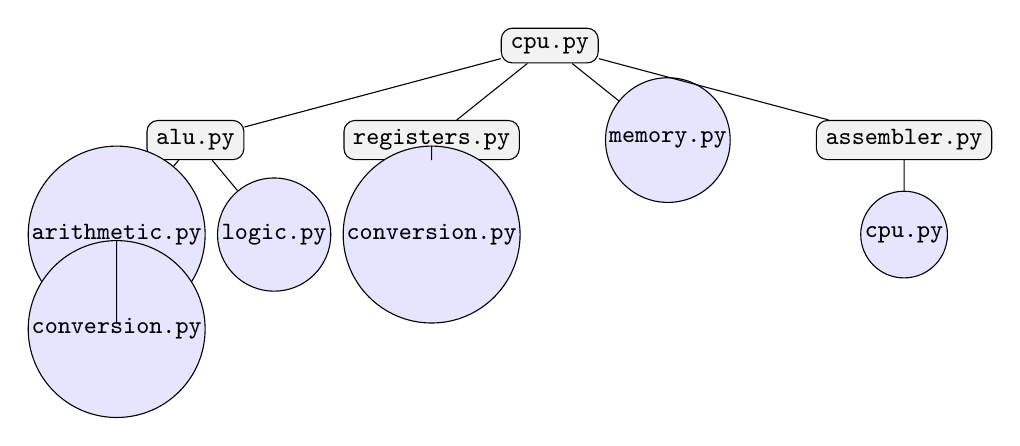
\begin{tikzpicture}[
    level distance=1.2cm,
    every node/.style={draw, rectangle, rounded corners, font=\ttfamily\small, fill=gray!10},
    level 1/.style={sibling distance=3cm},
    level 2/.style={sibling distance=2cm},
    level 3/.style={sibling distance=1.5cm},
    leaf/.style={draw, fill=blue!10, shape=circle, inner sep=1pt}
]
\node {\texttt{cpu.py}}
    child { node {\texttt{alu.py}}
        child { node[leaf] {\texttt{arithmetic.py}}
            child { node[leaf] {\texttt{conversion.py}} }
        }
        child { node[leaf] {\texttt{logic.py}} }
    }
    child { node {\texttt{registers.py}}
        child { node[leaf] {\texttt{conversion.py}} }
    }
    child { node[leaf] {\texttt{memory.py}} }
    child { node {\texttt{assembler.py}}
        child { node[leaf] {\texttt{cpu.py}} }
    };
\end{tikzpicture}
\caption{Simplified module dependency graph. \texttt{conversion.py} and \texttt{logic.py} are foundation modules with no Trinary dependencies.}
\label{fig:deps}
\end{figure}

\section{Memory Map}

The CPU uses a 512-address memory organised into four logical regions (Table~\ref{tab:memmap}). Addresses 0--127 hold program code and general data. Addresses 128--199 form the memory stack, growing downward from an initial stack pointer (SP) of 255. The video RAM occupies addresses 200--255, and the keyboard buffer sits at address 260.

\begin{table}[h]
\centering
\begin{tabular}{lll}
\toprule
Address range & Size & Purpose \\
\midrule
0--127   & 128  & General data / program storage \\
128--199 & 72   & Stack (grows down from SP=255) \\
200--255 & 56   & Video RAM (7 rows $\times$ 8 columns) \\
260      & 1    & Keyboard buffer \\
261--511 & 251  & Available \\
\bottomrule
\end{tabular}
\caption{Memory map for the default 512-address configuration.}
\label{tab:memmap}
\end{table}

For the Fantasy Console SDK path, an extended memory configuration with 10{,}000 addresses is used. This maps the SDK framebuffer (64 $\times$ 64 pixels) to addresses 1000--5095 and the SDK keyboard to 9000--9001.

\section{Number Representation}

All numeric values in the Trinary system use \emph{signed-magnitude} ternary representation. A positive number is written as a standard base-3 numeral; a negative number is prefixed with a minus sign. For example:

\begin{itemize}
    \item \texttt{"0"} = $0$
    \item \texttt{"10"} = $1 \times 3^1 + 0 \times 3^0 = 3$
    \item \texttt{"22"} = $2 \times 3^1 + 2 \times 3^0 = 8$
    \item \texttt{"-10"} = $-3$
    \item \texttt{"-22"} = $-8$
\end{itemize}

This representation is \emph{not} balanced ternary (which uses digits $-1, 0, +1$). The signed-magnitude convention was chosen for simplicity of implementation and familiarity to programmers accustomed to signed decimal notation. The conversion functions in \texttt{conversion.py} provide bidirectional mapping:

\begin{lstlisting}[language=Python, caption={Base conversion example}, label={lst:conversion}]
>>> from trinary.conversion import ternary_to_decimal, decimal_to_ternary
>>> ternary_to_decimal("102")
11
>>> ternary_to_decimal("-10")
-3
>>> decimal_to_ternary(11)
'102'
>>> decimal_to_ternary(-3)
'-10'
\end{lstlisting}

\section{Dual-Stack Design}

The Trinary CPU features two independent stacks serving different purposes.

\subsection{Memory Stack (PUSH / POP)}

The memory stack occupies addresses 128--199 (72 cells). The stack pointer (SP) starts at 255, above the memory-mapped region, and grows downward. Each PUSH decrements SP and stores a register value; each POP increments SP and loads a value into a register. The stack is bounded: pushing below address 128 raises \texttt{StackOverflowError}, and popping above 255 raises \texttt{StackUnderflowError}.

\begin{lstlisting}[language=Python, caption={Memory stack operation}, label={lst:memstack}]
# PUSH R0:  memory[SP] = R0; SP -= 1
# POP R0:   SP += 1; R0 = memory[SP]
#
# Initial: SP = 255
# After PUSH R0 (with R0=42): SP = 254, memory[255] = "42"
# After POP R1:             SP = 255, R1 = "42"
\end{lstlisting}

\subsection{Call Stack (CALL / RET)}

The CALL and RET instructions use a separate Python list (\texttt{call\_stack}) rather than memory-memory stack. CALL pushes the next instruction address onto the call stack and jumps to a target; RET pops the return address and resumes execution. This separation simplifies subroutine management and avoids conflating data storage with control flow.

\begin{lstlisting}[language=Python, caption={Call stack operation}, label={lst:callstack}]
# CALL target: call_stack.append(PC + 1); PC = target
# RET:         PC = call_stack.pop()
#
# Sequence at address 10: CALL 20
#   call_stack = [11], PC = 20
# Sequence at address 20: ... RET
#   call_stack = [], PC = 11
\end{lstlisting}

\section{Instruction Set Summary}

The Trinary CPU implements 26 instructions organised into 8 functional categories (Table~\ref{tab:isa}). Each instruction has a ternary opcode encoding (3 trits) and a variable number of operands depending on its format. A complete reference is provided in the companion document \texttt{docs/instruction-set.md}.

\begin{table}[h]
\centering
\begin{tabular}{llll}
\toprule
Category & Instructions & Format & Opcode range \\
\midrule
Data Movement & LOAD, MOV, CLR & C, A, B & 000--002 \\
Arithmetic    & ADD, SUB, MUL, DIV & A & 010--011, 122--200 \\
Logical       & AND, OR, NOT & A, B & 012--021 \\
Comparison    & CMP & A & 022 \\
Control Flow  & JMP, JZ, JNZ & D & 100--102 \\
Subroutines   & CALL, RET & D, E & 112, 120 \\
Stack         & PUSH, POP & B & 110--111 \\
Memory Access & STOREM, LOADM & M & 201--202 \\
Interrupts    & INT, IRET, EI, DI, SETIVT, SETTIMER & D, E, S, T & --- \\
System        & HALT & E & 121 \\
\bottomrule
\end{tabular}
\caption{Instruction set categories with assembly formats and ternary opcode ranges. Format codes: A (two-register), B (one-register), C (immediate), D (branch address), E (no operands), M (memory address), S (vector table), T (timer period).}
\label{tab:isa}
\end{table}

\section{Directory Structure}

The \texttt{src/trinary/} package is organised as follows:

\begin{lstlisting}[language=bash, caption={Package directory structure}, label={lst:dirs}]
src/trinary/
  conversion.py        # Trit class + base converters
  logic.py             # TNOT, TAND, TOR gates
  adder.py             # Native base-3 ripple-carry adder
  arithmetic.py        # ADD/SUB/MUL/DIV via decimal round-trip
  alu.py               # ALU: 8 operations + flag computation
  registers.py         # R0-R3 register file
  memory.py            # RAM with write hooks
  cpu.py               # CPU: 26 opcodes, 2 stacks, interrupts
  assembler.py         # Two-pass assembler
  machine.py           # Machine-code encoder/decoder
  os.py                # Interactive OS shell
  display/             # Text + framebuffer display
  sdk/                 # Fantasy Console SDK
  accelerator/         # Tensor coprocessor, GPU mode, SIMD
  hardware/            # Pipeline, cache, branch predictor, DMA, bus
  ui/                  # PyQt6 desktop visual simulator
  tal.py               # TAL structured-language compiler
  native/              # C backend (libternary.so)
\end{lstlisting}

\section{Exploring the Public API}

Listing~\ref{lst:explore-api} demonstrates how to import the package and inspect its major components.

\begin{lstlisting}[language=Python, caption={Exploring the Trinary public API}, label={lst:explore-api}]
from trinary.conversion import ternary_to_decimal, decimal_to_ternary
from trinary.logic import tnot, tand, tor
from trinary.alu import alu
from trinary.registers import RegisterFile
from trinary.memory import Memory
from trinary.cpu import CPU

# Base conversion
assert ternary_to_decimal("22") == 8
assert decimal_to_ternary(8) == "22"

# Logic gates
assert tnot(0) == 2
assert tand(1, 2) == 1
assert tor(0, 2) == 2

# ALU
result = alu("ADD", "10", "12")   # 3 + 5 = 8
assert result == "22"

# Register file
regs = RegisterFile()
regs.load("R0", "22")
assert regs.store("R0") == "22"

# Memory
mem = Memory(512)
mem.store(100, "102")
assert mem.load(100) == "102"

# CPU
cpu = CPU()
cpu.load_program(["LOAD R0 10", "LOAD R1 12", "ADD R0 R1", "HALT"])
cpu.run(verbose=False)
assert cpu.registers.store("R0") == "22"
\end{lstlisting}


\chapter{Environment Setup and Quick Start}

\section{Prerequisites}

The Trinary system requires Python 3.10 or later. Verify your Python version:

\begin{lstlisting}[language=bash, caption={Checking Python version}, label={lst:python-version}]
python --version
# Expected: Python 3.10.x or higher
\end{lstlisting}

Additional dependencies include \texttt{setuptools} for installation (bundled with Python), and optionally \texttt{PyQt6} for the graphical desktop interface and \texttt{pygame} for the Fantasy Console SDK audio/video.

\section{Package Installation}

Install the \texttt{trinary} package in editable mode from the project root. This links the source directory directly into your Python environment, so any edits to the source are immediately reflected without reinstallation.

\begin{lstlisting}[language=bash, caption={Installing the trinary package}, label={lst:install}]
cd trinary
pip install -e .
\end{lstlisting}

On Unix-like systems, the native C backend can be built for accelerated ALU operations:

\begin{lstlisting}[language=bash, caption={Building the native C backend (optional)}, label={lst:native-build}]
make -C src/trinary/native
# or: bash build_native.sh
\end{lstlisting}

\section{Running the Test Suite}

The project includes an extensive test suite covering every subsystem. Run all tests with pytest:

\begin{lstlisting}[language=bash, caption={Running the full test suite}, label={lst:tests}]
python -m pytest tests/ -v
\end{lstlisting}

This executes hundreds of tests across the conversion, logic, ALU, CPU, assembler, display, OS, SDK, accelerator, hardware simulation, and native backend modules. A successful run produces output similar to Figure~\ref{fig:test-output}.

\begin{figure}[h]
\centering
\begin{lstlisting}[basicstyle=\ttfamily\tiny, caption={Sample test output (abbreviated)}, label={lst:test-output}]
tests/test_conversion.py ..............                       [  2%]
tests/test_logic.py ...........                              [  4%]
tests/test_alu.py ..............                             [  6%]
tests/test_arithmetic.py ................                    [  9%]
tests/test_cpu.py ......................................... [ 16%]
...
tests/test_sdk.py ..............................               [ 85%]
tests/test_accelerator.py .................................. [ 95%]
tests/test_realistic_cpu.py ........                         [100%]
=== 572 passed in 12.34s ===
\end{lstlisting}
\caption{Abbreviated output from the full test suite.}
\label{fig:test-output}
\end{figure}

Subsets of tests can be run by module or keyword:

\begin{lstlisting}[language=bash, caption={Running specific test subsets}, label={lst:test-subsets}]
python -m pytest tests/test_cpu.py -v           # CPU-only tests
python -m pytest tests/test_sdk.py -v           # SDK tests
python -m pytest tests/ -k "accelerator" -v    # All accelerator tests
\end{lstlisting}

\section{Booting the Interactive OS Shell}

The legacy operating system shell provides an interactive environment running directly on the ternary CPU. Launch it with:

\begin{lstlisting}[language=bash, caption={Booting the interactive OS shell}, label={lst:os}]
python -m trinary.os
\end{lstlisting}

Upon boot, the OS clears the display, prints a banner showing the system version, and presents a command prompt (Figure~\ref{fig:os-boot}). The shell accepts commands typed at the keyboard buffer (address~260) and supports HELP, CLS, REGS (show registers), MEMDUMP, and RUN (execute a stored program).

\begin{figure}[h]
\centering
\begin{lstlisting}[basicstyle=\ttfamily\tiny]
Trinary OS v1.3.0
Ternary (Base-3) Computer System
512-word memory, 26 instructions, 2 stacks
Type HELP for commands
> HELP
Commands: HELP, CLS, REGS, MEMDUMP, RUN, HALT
>
\end{lstlisting}
\caption{OS shell boot screen and HELP output.}
\label{fig:os-boot}
\end{figure}

\section{Launching the PyQt6 Desktop UI}

The graphical visual simulator provides a complete debugging environment with syntax-highlighted assembly editor, register/memory inspectors, pipeline and cache visualizers, and performance dashboards. Launch it with:

\begin{lstlisting}[language=bash, caption={Launching the PyQt6 desktop UI}, label={lst:ui}]
pip install pyqt6          # if not already installed
python -m trinary.ui.app
\end{lstlisting}

The main window (Figure~\ref{fig:ui-main}) is organised into resizable panels. The left pane contains the assembly editor; the right pane shows machine code, registers, and flags. Lower panels display memory contents, stack state, execution trace, and the pixel framebuffer. A toolbar provides Assemble, Run, Step Into, Step Over, Reset, Pause, and Continue controls. A dropdown selector offers 13 built-in demo programs.

\section{Running Demo Programs}

The \texttt{demo\_programs} module provides pre-written assembly programs demonstrating various CPU features:

\begin{lstlisting}[language=bash, caption={Running demo programs}, label={lst:demos}]
python -m trinary.demo_programs
\end{lstlisting}

The launcher presents a numbered menu. Available demos include:

\begin{itemize}
    \item \textbf{Countdown}: Simple loop with decrement and conditional jump
    \item \textbf{Factorial}: Recursive factorial using CALL/RET
    \item \textbf{Fibonacci}: Iterative Fibonacci sequence
    \item \textbf{Timer Demo}: Program demonstrating the interrupt timer
    \item \textbf{Graphics Demo}: Drawing to the memory-mapped display
\end{itemize}

For the Fantasy Console SDK games (which use the 64$\times$64 pixel framebuffer), use the \texttt{demo\_games} launcher:

\begin{lstlisting}[language=bash, caption={Running Fantasy Console games}, label={lst:sdk-games}]
python -m trinary.demo_games pong        # Classic Pong
python -m trinary.demo_games snake       # Snake (TAL-compiled CPU assembly)
python -m trinary.demo_games breakout    # Breakout clone
python -m trinary.demo_games particles   # Particle system demo
python -m trinary.demo_games bouncing_logo  # Bouncing DVD-style logo
python -m trinary.demo_games tilemap     # Tilemap scroller
python -m trinary.demo_games rpg         # RPG overworld movement
\end{lstlisting}

\section{Viewing ASCII Architecture Diagrams}

The \texttt{diagrams} module prints system architecture diagrams directly to the terminal:

\begin{lstlisting}[language=bash, caption={Viewing architecture diagrams}, label={lst:diagrams}]
python -m trinary.diagrams
\end{lstlisting}

This displays a visual overview of the CPU architecture, memory layout, fetch-decode-execute cycle, and the complete system stack---providing a quick reference for the concepts covered in Chapter~2.

\section{Your First ``Hello, Ternary'' Program}

Listing~\ref{lst:hello-ternary} demonstrates the complete workflow: writing assembly source, assembling it into machine code, loading it onto the CPU, and executing it.

\begin{lstlisting}[language=Python, caption={Writing, assembling, and running a ``Hello, Ternary'' program}, label={lst:hello-ternary}]
from trinary.cpu import CPU
from trinary.assembler import Assembler

# Write assembly source
source = """
start:
    LOAD R0 10       # R0 = 3 (ternary "10")
    LOAD R1 12       # R1 = 5 (ternary "12")
    ADD R0 R1        # R0 = 3 + 5 = 8 (ternary "22")
    STOREM 100 R0    # Store result at address 100
    HALT
"""

# Assemble
assembler = Assembler()
program = assembler.assemble(source)
print("Assembled program:", program)

# Load and run
cpu = CPU()
cpu.load_program(program)
cpu.run(verbose=True)

# Inspect result
result = cpu.memory.load(100)
print(f"Result at memory[100]: {result}")
# Expected: "22" (ternary for 8)
\end{lstlisting}

When executed, the verbose mode prints a step-by-step trace:

\begin{lstlisting}[basicstyle=\ttfamily\small, caption={Execution trace for the Hello Ternary program}, label={lst:trace}]
Step  PC  Instruction       R0   R1   R2   R3
----- --- ----------------- ---- ---- ---- ----
  0    0  LOAD R0 10         3    0    0    0
  1    1  LOAD R1 12         3    5    0    0
  2    2  ADD R0 R1          8    5    0    0
  3    3  STOREM 100 R0      8    5    0    0
  4    4  HALT               8    5    0    0
Result at memory[100]: 22
\end{lstlisting}

This simple program demonstrates four instruction categories in action: data movement (LOAD), arithmetic (ADD), memory access (STOREM), and system control (HALT). The following chapters will examine each of these categories, and every CPU mechanism, in detail.
